\section*{Section 203 of the Voting Rights Act}

\begin{figure*}[h]
	\centering
	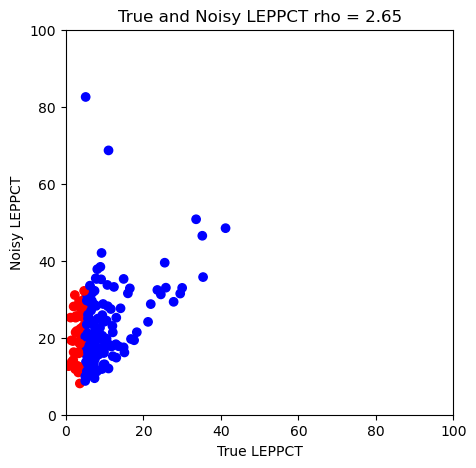
\includegraphics[width=0.5\linewidth]{images/true_noisy_leppct_2.65}
	\caption{LEPPCT vs. LEPPCT noisy values after DP mechanism at $\rho=2.65$}
	\label{fig:leppct}
\end{figure*}


Section 203 of the Voting Rights Act requires certain jurisdictions to provide bilingual election materials and
assistance to voters who are not proficient in English. To determine which jurisdictions are covered by this provision,
the Census Bureau collects data on the number and percentage of voting-age citizens who are members of a language
minority group and have limited English proficiency.

The Census Bureau uses three measures to calculate these numbers: the Limited English Proficient Population Count
(LEPPCT), the Illiteracy Rate (ILLRAT), and the Voting Age Citizen Language Minority Group Citizen Voting Age
Population (VACLEP).

The LEPPCT is the percentage of people in a language minority group who have limited English proficiency. The ILLRAT
is the rate of total LMG voting age citizens who are limited-English proficient and have less than a 5th grade
education. The VACLEP is the number of voting-age citizens who are members of a language minority group.

By using these three measures, the Census Bureau determines which jurisdictions meet the criteria for coverage under
Section 203. This information is then used by election officials to provide bilingual election materials and assistance
to voters who need it, ensuring that everyone has an equal opportunity to participate in the electoral process.

\subsection*{Allocation Formula}
Coverage from Section 203 is determined by a simple mechanism that ensures that a county satisfies the following conditions:

The ILLRAT is greater than the national illiteracy rate AND the LEPPCT is greater than 5\% OR the VACLEP is greater than
10,000. There are further nuances in this computation for American Indian and Alaska Native areas which we will refer
to \cite{Census203}.

\subsection*{Analysis}
In figure \ref{fig:leppct}, we observe the effects of applying differential privacy to the population counts in a similar
way to our approach in the Title I misallocations. We observe that applying DP noise can lead to false negative
outcomes, where communities that would originally receive coverage from Section 203 would be denied because their noisy
LEPPCT value would not satisfy the threshold constraints
